\begin{figure}[h!]
	\centering
	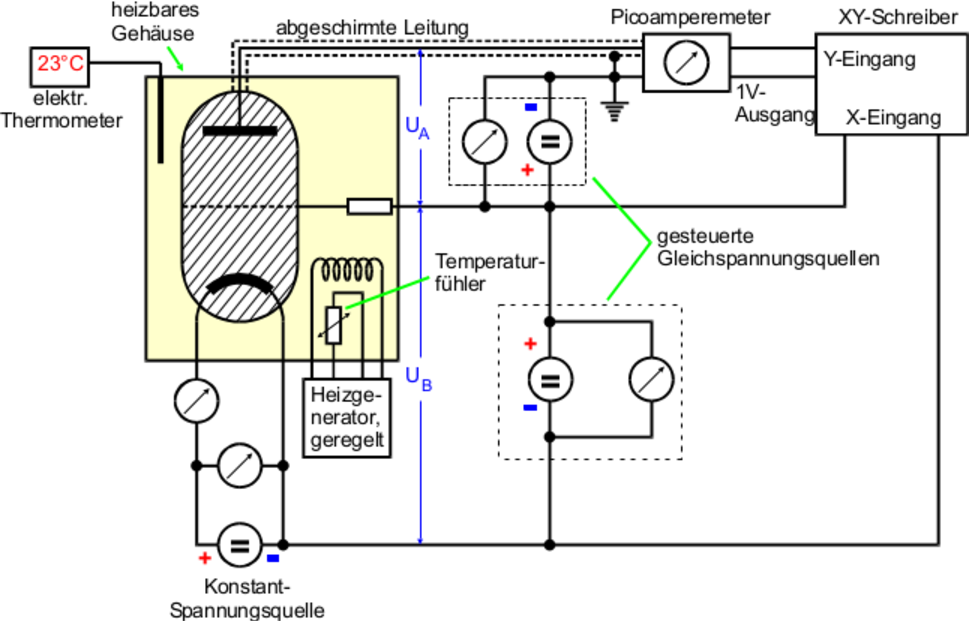
\includegraphics[width = 0.85\textwidth]{Aufbau_Schaltbild.pdf}
	\caption{Schaltbild zur Aufnahme einer Franck-Hertz-Kurve}
	\label{fig:Schaltbild}
\end{figure}


Abbildung \ref{fig:Schaltbild} zeigt den verwendeten Versuchsaufbau. Gelb hinterlegt ist der schematische Aufbau aus Kapitel \ref{sec:Aufbau_Grund}. Die einzige Erweiterung stellt der XY-Schreiber dar, mit dem verschiedene Kurven aufgezeichnet werden sollen.
\subsubsection*{Die Messung}
Die Messung besteht aus der Aufzeichnung verschiedener Kurven mit dem XY-Schreiber. \\
Die erste Kurve ist $I_\text{A}(U_\text{A})$. Sie wird bei konstanter Beschleunigungsspannung
\begin{align}
	U_\text{B} = \SI{11}{\volt}
\end{align}
und jeweils einmal bei einer Temperatur von $T=\SI{25}{\celsius}$ und $T=\SI{130}{\celsius}$ aufgenommen. \\
Dann wird die Franck-Hertz-Kurve $I_\text{A}(U_\text{B})$, mit konstanter Bremsspannung
\begin{align}
	U_\text{A} = \SI{1}{\volt}
\end{align}
bei einer Temperatur von $T = \SI{100}{\celsius}$. \\
Zuletzt wird zur Bestimmung der Ionisierungsenergie eine (nun beschleunigende) Spannung
\begin{align}
	U_\text{A} = \SI{30}{\volt}
\end{align}
angelegt und wieder $I_\text{A}(U_\text{B})$ aufgetragen.